% !TeX encoding = utf8
% !TeX program = xelatex
% !BIB program = bibtex
%
% Configuration options:
% english - Use for English language theses
% german - Use for German language theses
% ba - Use for Bachelor theses
% ma - Use for Master theses
\documentclass[german,ba]{tudo-sse-thesis}

% Add the packages necessary
\usepackage[math]{blindtext}

% Provide your title
\subtitle{Optimierung rekonfigurierbarer Netzwerke für Bulk-Transfers mit gängigen Scheduling-Algorithmen in Mininet}

% Provide your name
\author{Julian Huhn}

% Provide examiner names. First examiner has a reasonable default and only needs to changed if the default does not fit.
\firstexaminer{Prof.\ Dr.\ Dr.\ Klaus-Tycho Förster}
\secondexaminer{Prof.\ Dr.\ Peter Buchholz}

\begin{document}

\maketitle

\pagenumbering{roman}

% Only add for english documents
%\begin{abstract}
%  This is an Abstract. %\blindtext
%\end{abstract}

% This needs to be in German or English documents
%\begin{abstract-ger}
%  Dies ist eine Zusammenfassung.  ßäöü %\blindtext
%\end{abstract-ger}

\tableofcontents
\cleardoublepage

\pagenumbering{arabic}

% Add your content here
\chapter{Motivation}

\section{Herausforderungen moderner Rechenzentren}
\chapter{Grundlagen}

\section{Rekonfigurierbare Netzwerke}

\subsection{Optical Circuit Switching}

\subsection{Algorithmen zur Konfiguration von rekonfigurierbaren Netzwerken mit Optical Circuit Switching}

z.B.: Maximal Matching (Graph Theorie), Greedy (größte Kante für größten Transfer), ...

\section{Bulk-Transfers}

Kriterien für Bulk Transfers

Wann ist ein Bulk-Transfer gut und wann schlecht?

\section{Scheduling-Algorithmen}

Überblicksartikel über Scheduling-Algorithmen zitieren für die Eingrenzung

\section{Mininet}

\subsection{IPMininet}

https://dial.uclouvain.be/pr/boreal/object/boreal%3A235433/datastream/PDF_01/view

\section{Weitere Arbeiten und Eingrenzung}
\chapter{Experimentelle Untersuchungen in Mininet}

\section{Voruntersuchungen}

\section{Methodik}

\section{Topologien}

\section{Ergebnisse}
\chapter{Diskussion}
\chapter{Ausblick}


% Bibliography
\bibliographystyle{ACM-Reference-Format}
\bibliography{bibliography/references}
\addcontentsline{toc}{chapter}{\bibname}

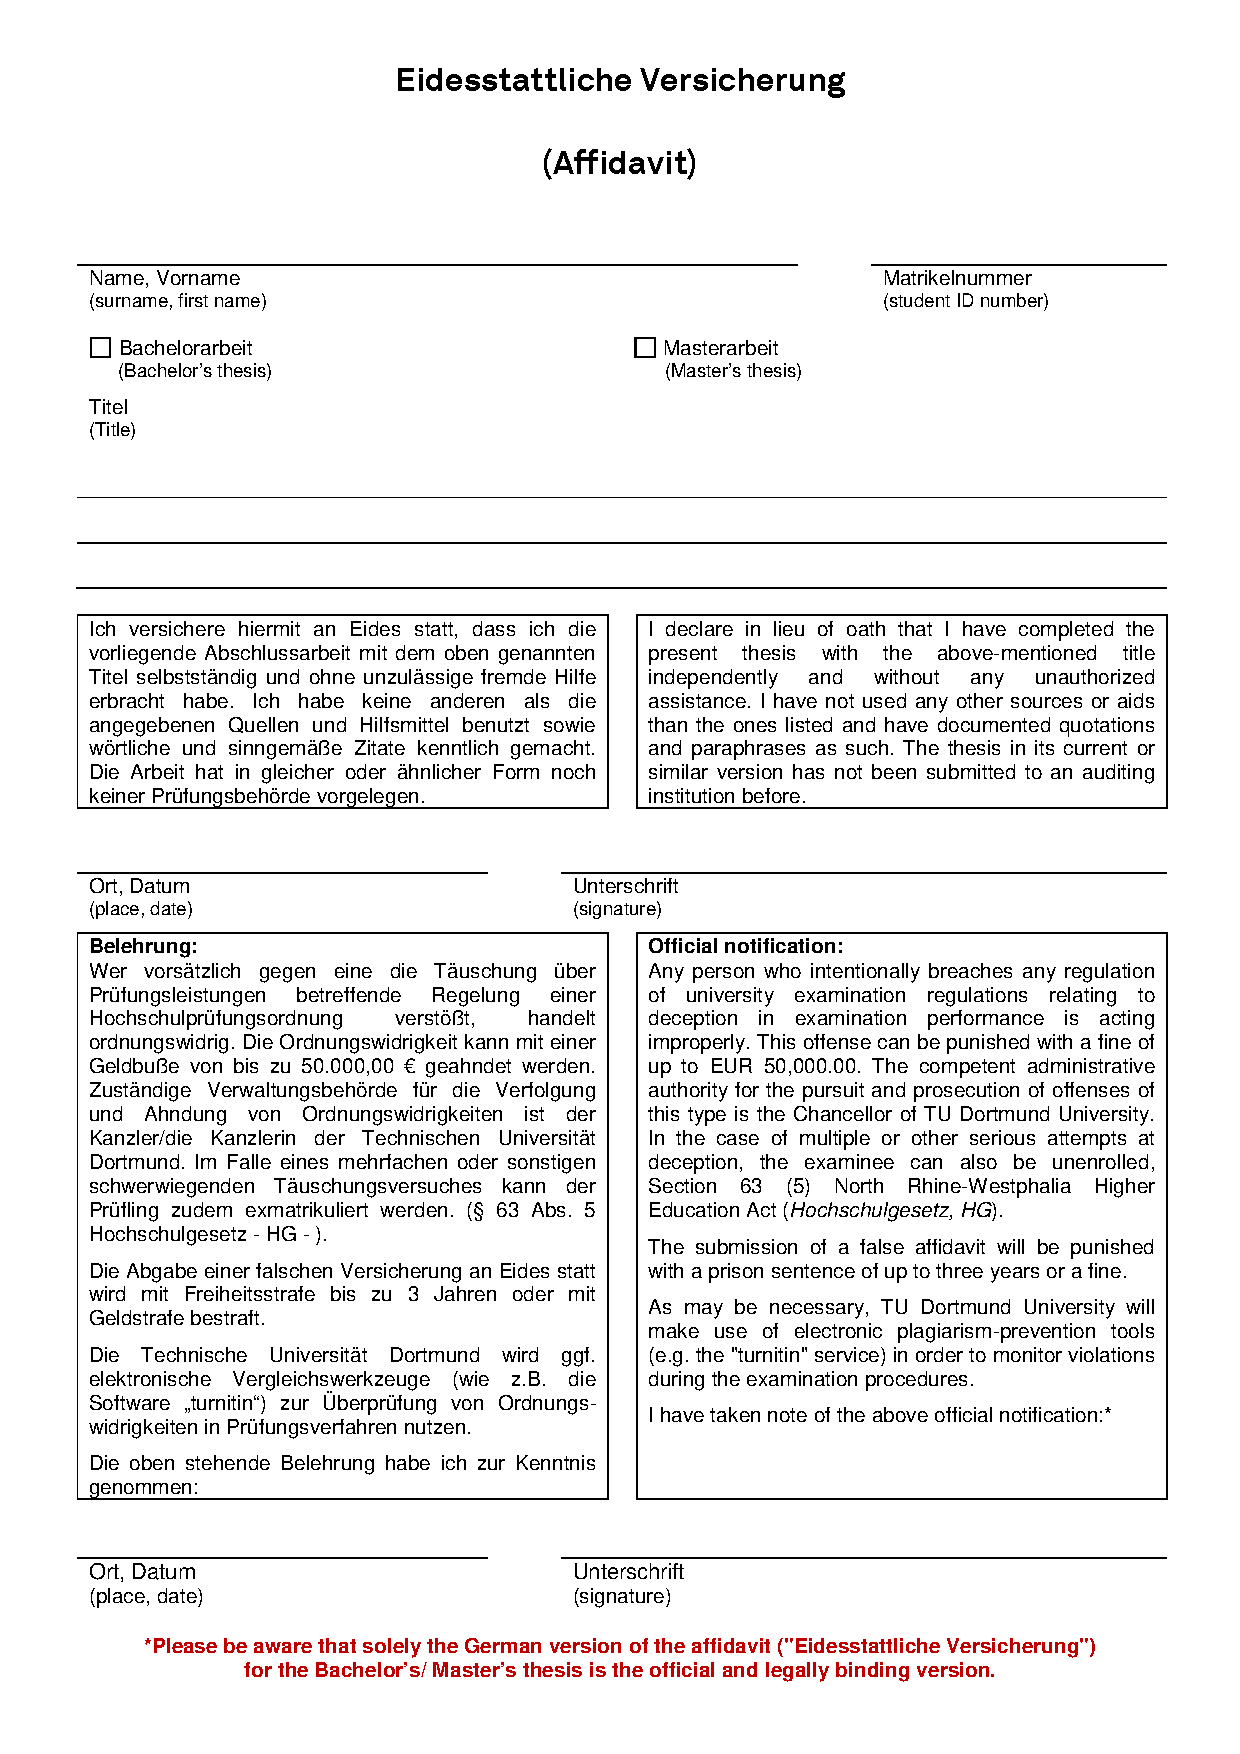
\includepdf[pages=-]{Eidesstattliche_Versicherung}

\end{document}
